\documentclass{article}

\usepackage{graphicx}
\usepackage{booktabs} % for table /toprule, /midrule, etc
\usepackage{amsmath}

\title{Controller parameter identification using direct collocation}

\begin{document}

\maketitle

\section{Introduction}

Given a mathematical model of a system operating inside a closed loop system
and experimental measurements of data collected from that system, it is common
to attempt to identify parameters of the mathematical model that cause the
models response to the measured inputs to best fit the measured output data.
For linear systems, there are a variety of solutions to these identification
problems, but for non linear systems the solution amounts to solving a
optimization problem which is most certinaly laden with many local optima.

We are particularly interested in identifying the parameters of the controller
in a closed loop system. It is theorized that creatures operate, at least
partially, under a closed loop during locomotion. Humans for example have
proprioceptive, vestibular, etc sensors that provide a rich set of internal
measurements that guide our choice for muscle activation. If the map from
sensastion to acuatation can be identified, then the engineer will have a
mathematical model of the highly evolved control system human's employ that can
be used for biomicry in robotic controls. This is potentially useful for
humanoid robots and assitive devices for both able body and disabled
locomoters.

In this paper, we present the use of direct collocation to identify the
controller parameters of controled inverted pendulum that is excited by
pseudo-random external inputs. The method is compared to more traditional
shooting optimization methods and also a direct identification method.

Direct collocation is more commonly used to find the open loop controls that
drive a mathematical model to track a particular trajectory.

\section{Closed Loop System Model Description}

Herein we make use of a well known and studied planar inverted pendulum on a
cart as a our plant model, except that we allow any number of links. The cart
with mass, $m_o$ can move laterally but is restricted to the origin by a linear
spring and damper. The links are masseless and there is a point mass located at
each link joint. The external loads acting on the system are a lateral force
which acts on the cart and ``joint torques'' at each joint which apply an equal
and opposite torque between the adjacent joints.

% TODO : m_{n+1} and q_{n+1} should be m_n and q_n in the figure. And l_n
% should be l_{n-1} if n is the number of links.

\begin{figure}
  \centering
  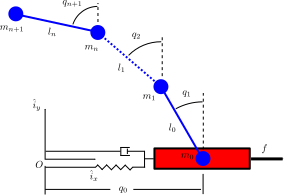
\includegraphics{figures/n-pendulum-with-cart.pdf}
  \caption{Free body diagram of the n-link pendulum on a cart used in this
    study.}
  \label{fig:free-body-diagram}
\end{figure}

\begin{table}
  \centering
  \caption{Constant parameters in the plant}
  \begin{tabular}{llll}
    \toprule
    Variable   & Description                          & Value            & Units \\
    \midrule
    $n$        & number of links                      & 1-4              & NA    \\
    $m$        & mass                                 & $75.0 / (n + 1)$ & kg    \\
    $l$        & length of each link                  & $1.75 / n$       & m     \\
    $c$        & lateral spring damping coefficient   &                  & Ns/m  \\
    $k$        & lateral spring stiffness coefficient &                  & N/m   \\
    \bottomrule
  \end{tabular}
\end{table}

To close the loop, we assume full state feedback and make use of an infinite
horizon continous time linear quadratic regulator to compute the optimal
feedback gains to stabilize the linearized form of the equations about the
nominal operating point, $q,u=0$. Since we are not concerned with performance,
we simply set the $Q$ and $R$ matrices to the appropriate sized identify
matrix.

% TODO : Maybe include a table of gains for the the 1, 2, 3 and 4 link
% pendulums in the Appendix.

For example the open loop equations of motion for the 1 link pendulum take the
following form:

\begin{equation}
   \begin{bmatrix}
     0 \\ 0 \\ 0 \\ 0
   \end{bmatrix}
   =
   \begin{bmatrix}
     \dot{q}_{0} - u_{0} \\
     \dot{q}_{1} - u_{1} \\ c u_{0} + k q_{0} + l_{0} m_{1} u^{2}_{1}
     \operatorname{sin}\left(q_{1}\right) - l_{0} m_{1}
     \operatorname{cos}\left(q_{1}\right) \dot{u}_{1} + \left(m_{0} +
     m_{1}\right) \dot{u}_{0} - F \\
     -g l_{0} m_{1} \operatorname{sin}\left(q_{1}\right) + l_{0}^{2} m_{1} \dot{u}_{1} - l_{0} m_{1} \operatorname{cos}\left(q_{1}\right) \dot{u}_{0} - T_{1}
   \end{bmatrix}
\end{equation}

% TODO : Show a block diagram of the system

The loop is closed by replacing the joint torque with

\begin{align}
   u^{con} = \mathbf{K} (x_{eq} - x) \\
   u^{con} = T_{1} = -k_{00} q_0 - k_{01} q_1 - k_{02} u_0 - k_{03} u_1
\end{align}

We excite the system at $F$ with a sum of sines to create a pseudo-random
input. And add two types of noise to the system: process $w$ and measurement
$y$.

\begin{align}
  \dot{x} = f(x, u) + w(t) \\
  y = x + v(t)
\end{align}

\end{document}
